

\captionsetup[figure]{labelformat=simple, labelsep=colon}
\captionsetup[table]{labelformat=simple, labelsep=colon}
\renewcommand{\thefigure}{S\arabic{figure}}
\renewcommand{\thetable}{S\arabic{table}}

\setcounter{figure}{0}
\setcounter{table}{0}

\onehalfspacing
\pagenumbering{arabic}
\setcounter{1}

\section*{\LARGE Supporting Information}



\section{Prediction Powered Inference (PPI)}\label{sec:power}

\subsection{PPI Standard Error and Correlation}\label{sec:ppi-se-and-corr}

In this section, we will define the PPI correlation $\tilde{\rho}$ and show that the standard error of the PPI estimator $\hat{\theta}^{\PPI}$ is equal to 
\begin{equation}\label{eq:PPI-se-supp}
    \mathrm{SE}(\hat{\theta}^{\PPI}) = \frac{\sigma}{\sqrt{n}}\sqrt{1-\frac{N}{N+n}\tilde{\rho}^2}.
\end{equation}
This expression for the standard error is given in equation~\eqref{eq:PPI-se} and used in our power analysis. To define $\tilde{\rho}$ and prove equation~\eqref{eq:PPI-se-supp}, we will use some results and concepts from \cite{angelopoulos2024ppi}. In particular, equation~\eqref{eq:PPI-se-supp} only holds when $\hat{\theta}^{\PPI}$ is the \emph{power-tuned} PPI estimator -- a concept introduced in \cite[Section 6]{angelopoulos2024ppi} and reviewed here.

Let $\{(X_i,Y_i)\}_{i=1}^n$ and $\{\widetilde{X}_i\}_{i=1}^N$ be the labeled and unlabeled datasets as in Section~\ref{sec:PPI}. Let $f$ be the machine learning algorithm that predicts $Y$ from $X$. Let $\ell_\theta(x,y)$ be a loss function with $\theta \in \reals^d$. The loss function $\ell_\theta$ defines an estimand $\theta^\star$ by
\[\theta^\star = \argmin_{\theta \in \reals^d} \mathbb{E}[\ell_\theta(X,Y)]. \]
For example, if $\ell_\theta(x,y) = \frac{1}{2}(x^\top \theta - y)^2$, then $\theta^\star$ is the vector of ordinary least squares coefficients for regressing $Y$ on $X$. 

\cite{angelopoulos2024ppi} introduce a family of estimators $\hat{\theta}^{\PPI}_\lambda$ for $\theta^\star$. These estimators depend on a tuning parameter $\lambda \in \reals$ and are given by
\[
    \hat{\theta}_{\lambda}^\PPI = \argmin_{\theta \in \reals^d}\frac{1}{n}\sum_{i=1}^n \ell_\theta(X_i,Y_i) + \lambda\left(\frac{1}{N}\sum_{i=1}^N \ell_\theta(\widetilde{X}_i,f(\widetilde{X}_i)) - \frac{1}{n}\sum_{i=1}^n \ell_\theta(X_i, f(X_i)\right). 
\]
Taking $\lambda = 0$ corresponds to the classical M-estimator for $\theta^\star$
\[
    \hat{\theta}^{\mathrm{classical}} =\hat{\theta}^\PPI_0 = \argmin_{\theta \in \reals^d} \frac{1}{n}\sum_{i=1}^n \ell_\theta(X_i,Y_i). 
\]
In Theorem~1 of \cite{angelopoulos2024ppi}, the authors show that, under certain assumptions of the loss $\ell_\theta$, the PPI estimator $\hat{\theta}^{\PPI}_\lambda$ satisfies a central limit theorem. Specifically, if $n,N \to \infty$ with $n/N \to r$, then
\begin{equation}
    \label{eq:CLT}   
    \sqrt{n}\left(\hat{\theta}^\PPI_\lambda - \theta^\star\right) \stackrel{d}{\to} \mathcal{N}(0,\Sigma^\lambda),
\end{equation}
where $\mathcal{N}(\mu,\Sigma)$ denoted the $d$-dimensional Guassian distribution with mean $\mu$ and covariance matrix $\Sigma$. The asymptotic covariance matrix $\Sigma^\lambda$ has the following ``sandwich'' form
\begin{align}
    \Sigma^{\lambda} =& H^{-1}_{\theta^\star}\cov(\nabla \ell_{\theta^\star})H^{-1}_{\theta^\star}+\lambda^2(1+r) H^{-1}_{\theta^\star}\cov(\nabla \ell_{\theta^\star}^f )H^{-1}_{\theta^\star}\nonumber \\
    &- \lambda H^{-1}_{\theta^\star}\left(\cov(\nabla \ell_{\theta^\star}^f,\nabla\ell_{\theta^\star})+\cov(\nabla \ell_{\theta^\star},\nabla\ell_{\theta^\star}^f)\right)H^{-1}_{\theta^\star},\label{eq:cov-matrix}
\end{align}
where $\nabla \ell_{\theta^\star}$ is the gradient of $\ell_\theta(X,Y)$ with respect to $\theta$ evaluated at $\theta^\star$, $\nabla \ell_{\theta^\star}^f$ is the gradient of $\ell_\theta(X,f(X))$ evaluated at $\theta^\star$ and $H_\theta^\star = \E[\nabla^2 \ell_{\theta^\star}(X,Y)].$

By equation~\eqref{eq:CLT} the standard error of the $j$th coordinate $\hat{\theta}^{\PPI}_{\lambda,j}$ is $\sqrt{\Sigma^{\lambda}_{j,j}/n}$. We will show that if $\lambda$ is chosen by \emph{power tuning} \citep[Section~6]{angelopoulos2024ppi}, then the PPI standard error will simplify to the expression in \eqref{eq:PPI-se-supp}.

Power tuning \citep[Section~6]{angelopoulos2024ppi} chooses $\lambda$ to minimize $\Sigma_{j,j}^\lambda$. This is equivalent to choose $\lambda$ to minimize the standard error of $\hat{\theta}^{\PPI}_{\lambda,j}$. From \eqref{eq:cov-matrix}, we have
\begin{align*}
    \Sigma^{\lambda}_{j,j} &= \left[H^{-1}_{\theta^\star}\cov(\nabla \ell_{\theta^\star})H^{-1}_{\theta^\star}\right]_{j,j}+\lambda^2(1+r) \left[H^{-1}_{\theta^\star}\cov(\nabla \ell_{\theta^\star}^f )H^{-1}_{\theta^\star}\right]_{j,j} \\
    &- \lambda \left[H^{-1}_{\theta^\star}\left(\cov(\nabla \ell_{\theta^\star}^f,\nabla\ell_{\theta^\star})+\cov(\nabla \ell_{\theta^\star},\nabla\ell_{\theta^\star}^f)\right)H^{-1}_{\theta^\star}\right]_{j,j}\\
    &=\left[H^{-1}_{\theta^\star}\cov(\nabla \ell_{\theta^\star})H^{-1}_{\theta^\star}\right]_{j,j}
    +\lambda^2 (1+r) \left[H^{-1}_{\theta^\star}\cov(\nabla \ell_{\theta^\star}^f)H^{-1}_{\theta^\star}\right]_{j,j}\\
    &- 2\lambda \left[H^{-1}_{\theta^\star}\cov(\nabla \ell_{\theta^\star}^f,\nabla\ell_{\theta^\star})H^{-1}_{\theta^\star}\right]_{j,j}.
\end{align*}
To get the final expression, we have used that $\cov(\nabla \ell_{\theta^\star}^f,\nabla \ell_{\theta^\star})^\top = \cov(\nabla \ell_{\theta^\star},\nabla \ell_{\theta^\star}^f)$ and that $H_{\theta^*}^{-1}$ is symmetric. The function $\lambda \mapsto \Sigma_{j,j}^\lambda$ is quadratic in $\lambda$ and its minimum occurs at
\[
    \lambda^\star_j = \frac{1}{1+r}\frac{\left[H^{-1}_{\theta^\star}\cov(\nabla \ell_{\theta^\star}^f,\nabla\ell_{\theta^\star})H^{-1}_{\theta^\star}\right]_{j,j}}{\left[H^{-1}_{\theta^\star}\cov(\nabla \ell_{\theta^\star}^f)H^{-1}_{\theta^\star}\right]_{j,j}}. 
\]
Furthermore, when $\lambda = \lambda^\star_{j}$, we have
\begin{align*}
    \Sigma^{\lambda^\star_j}_{j,j} =&  \left[H^{-1}_{\theta^\star}\cov(\nabla \ell_{\theta^\star})H^{-1}_{\theta^\star}\right]_{j,j}\\
    &\times \left( 1 - \frac{1}{1+r}\frac{\left[H^{-1}_{\theta^\star}\cov(\nabla \ell_{\theta^\star}^f,\nabla\ell_{\theta^\star})H^{-1}_{\theta^\star}\right]_{j,j}^2}{\left[H^{-1}_{\theta^\star}\cov(\nabla \ell_{\theta^\star}^f)H^{-1}_{\theta^\star}\right]_{j,j}\left[H^{-1}_{\theta^\star}\cov(\nabla \ell_{\theta^\star})H^{-1}_{\theta^\star}\right]_{j,j}}\right) \\
    =&\sigma^2_j\left(1-\frac{1}{1+r}\tilde{\rho}^2_j\right),
\end{align*}
where we have defined $\sigma^2_j = \left[H^{-1}_{\theta^\star}\cov(\nabla \ell_{\theta^\star})H^{-1}_{\theta^\star}\right]_{j,j}$ and
\begin{equation}\label{eq:PPI_corr}
    \tilde{\rho}^2_j =   \frac{\left[H^{-1}_{\theta^\star}\cov(\nabla \ell_{\theta^\star}^f,\nabla\ell_{\theta^\star})H^{-1}_{\theta^\star}\right]_{j,j}^2}{\left[H^{-1}_{\theta^\star}\cov(\nabla \ell_{\theta^\star}^f)H^{-1}_{\theta^\star}\right]_{j,j}\left[H^{-1}_{\theta^\star}\cov(\nabla \ell_{\theta^\star})H^{-1}_{\theta^\star}\right]_{j,j}}.
\end{equation}
The quantity $\sigma_j^2$ is the asymptotic variance of the classical estimator $\hat{\theta}^{\mathrm{classical}}$ and $\tilde{\rho}_j$ is the PPI correlation. 

Since $r=\frac{n}{N}$, the standard error of $\hat{\theta}^{\PPI}_{\lambda^\star_j,j}$ from a sample of $n$ labeled data points and $N$ unlabeled data point is
\[
   \mathrm{SE}(\hat{\theta}^{\PPI}_{\lambda^\star_j, j})= \sqrt{\Sigma_{j,j}^{\lambda^\star_j}/n} = \frac{\sigma_j}{\sqrt{n}}\sqrt{1-\frac{N}{N+n}\tilde{\rho}^2_j}.  
\]
In practice, $\lambda^\star_j$ has to be estimated. \cite{angelopoulos2024ppi} provide a consistent estimator $\hat{\lambda}_j$ for $\lambda^\star_j$ and show that $\hat{\theta}_{\hat{\lambda}_j,j}^{\PPI}$ achieves the same asymptotic variance as $\hat{\theta}^{\PPI}_{\lambda^\star_j,j}$. 

To simplify notation, we will write $\hat{\theta}^{\PPI}$ for $\hat{\theta}^{\PPI}_{\hat{\lambda}_j,j}$ and $\sigma$ instead of $\sigma_j$ and $\tilde{\rho}$ instead of $\tilde{\rho}_j$. With this notation we have
\[ 
    \mathrm{SE}(\hat{\theta}^{\PPI}) = \frac{\sigma}{\sqrt{n}}\sqrt{1-\frac{N}{N+n}\tilde{\rho}^2},
\]
as claimed in equations~\eqref{eq:PPI-se} and \eqref{eq:PPI-se-supp}.

\subsection{The Effective Sample Size in PPI}\label{sec:effective-sample-size}

The \emph{effective sample size} is the number $n_0$ of labeled data points that would give the same standard error of using PPI with $n$ labeled points and $N$ unlabeled points. The standard error with $n_0$ labeled data points is simple $\sigma/\sqrt{n_0}$. Equating this with the PPI standard error in \eqref{eq:PPI-se-supp} gives
\[
    n_0 = n \cdot \frac{n+N}{n+N-N\tilde{\rho}^2}. 
\]
Let $k = \frac{N}{n}$. Then, the effective sample size in PPI increases the number of human subjects by a factor of 
\[ 
    \frac{1+k}{1+k-k\tilde{\rho}^2} \ge 1.
\]
When $\tilde{\rho}^2=1$, this factor equals $1+k$ and the effective sample size is $n(1+N/n)=n+N$. That is, the effective sample size is the size of the full pooled sample. When $\tilde{\rho}=0$, this factor equals $1$ and the effective sample size is $n$ meaning that only the labeled samples are used.


\subsection{The Cost of PPI and Classical Inference}

In this section we derive the percentage of cost saved by PPI as reported in Figure~\ref{fig:perc-cost-reduction}. This is done by first finding all pairs of sample sizes $(n,N)$ that achieve the same standard error as a baseline classical experiment with $n_0$ labeled data points. Then, given the costs of collecting a labeled and unlabeled sample, we find the optimal pair $(n^\star,  N^\star)$ that minimizes the cost of PPI while still having the same power as the baseline classical experiment. The results in this section are used in the next two sections to derive the cheapest pair and most powerful pair for our power analysis.

Let $S(n,N)$ be the standard error of the PPI estimate, so that
\[
    S(n,N) = \frac{\sigma}{\sqrt{n}}\sqrt{1- \frac{N}{N+n}\tilde{\rho}^2}. 
\]
In a baseline experiment $n_0$ labeled samples, the standard error is $S(n_0, 0) = \sigma/\sqrt{n_0}$. By rearranging the equation $S(n,N) = \sigma/\sqrt{n_0}$, it can be shown that $S(n,N)=\sigma/\sqrt{n_0}$ if and only if 
\begin{equation}
n_0(1-\tilde{\rho}^2) < n \le n_0 \quad \text{and} \quad
    N = \frac{n(n_0 - n)}{n-n_0(1-\tilde{\rho}^2)} .\label{eq:level curves}
\end{equation}
Let $c_X$ and $c_Y$ be the cost of collecting $X$ and $Y$ and let $c_f$ be the cost of computing $f(X)$.  The cost of performing PPI with $n$ labeled subjects and $N$ unlabeled subjects is 
\begin{equation*}
    C(n,N) = (c_X+c_Y+c_f)n + (c_X+c_f)N.
\end{equation*}
This is because PPI requires $X_i$, $Y_i$, and $f(X_i)$ for the $n$ labeled samples and requires $\widetilde{X}_i$ and $f(\widetilde{X}_i)$ for the $N$ unlabeled samples. If we let $\gamma = (c_X+c_f)/c_Y$, then
\begin{equation*}
    C(n,N) = c_Y((1+\gamma) n + \gamma N)
\end{equation*}


Our goal is to find the pair $(n^\star, N^\star)$ that satisfies the constraints in equation~\eqref{eq:level curves} and minimizes $C(n,N)$. That is, $(n^\star, N^\star)$ is the solution to the optimization problem
\begin{equation}
\begin{array}{ll}
        \mbox{minimize} & C(n,N)\\
        \mbox{subject to} & \mbox{equation }\eqref{eq:level curves}
    \end{array}
\end{equation}
This optimization problem can be solved by first substituting $N=\frac{n(n_0-n)}{n-n_0(1-\tilde{\rho}^2)}$ into $C(n,N)$. This gives the cost as a function of $n$ alone. Setting the derivative of this function equal to zero gives
\begin{equation}\label{eq:nstar}
    n^\star = n_0\left(1-\tilde{\rho}^2+\sqrt{\gamma \tilde{\rho}^2(1-\tilde{\rho}^2)}\right)\quad \text{and} \quad N^\star =   \frac{n^\star(n_0-n^\star)}{n^\star - (1-\tilde{\rho}^2)n_0}.
\end{equation}
At the optimal pair $(n^\star, N^\star)$, the cost is 
\begin{equation}\label{eq:best-cost}
    C(n^\star, N^\star) = c_Y n_0\left(1-\tilde{\rho}^2 + \gamma\tilde{\rho}^2 +2\sqrt{\gamma \tilde{\rho}^2(1-\tilde{\rho}^2)} \right). 
\end{equation}
In contrast, the cost of performing classical inference with $n_0$ human subjects is 
\[
    C_0(n_0) = (c_Y+c_X)n_0. 
\]
This equation for the costs in classical inference is simpler since we do not need to compute $f(X_i)$ on the labeled data. It follows that PPI is more cost-effective than classical inference if and only if 
\[
c_Y \left(1-\tilde{\rho}^2 + \gamma\tilde{\rho}^2 +2\sqrt{\gamma \tilde{\rho}^2(1-\tilde{\rho}^2)} \right) \le c_Y+c_X.
\]
Furthermore, when this condition is satisfied, the optimal \emph{absolute} cost savings from PPI are
\[
C_0(n_0) - C(n^\star, N^\star) = n_0(c_X + c_Y(\tilde{\rho}^2 - \gamma \tilde{\rho}^2 - 2 \sqrt{\gamma \tilde{\rho}^2 (1-\tilde{\rho}^2)})).
\]
The \emph{relative} cost savings from PPI are 
\[
\frac{C_0(n_0)-C(n^\star, N^\star)}{C_0(n_0)} = \frac{c_X}{c_Y} + \tilde{\rho}^2 - \gamma \tilde{\rho}^2 - 2 \sqrt{\gamma \tilde{\rho}^2(1-\tilde{\rho}^2)}.
\]
In the context of mixed subjects experiments, it is natural to take $c_X=0$. This is because $c_X$ is simply the cost of recording demographic information or treatment assignments which is small compared to the cost of the full survey. When $c_X=0$, we have $\gamma = c_f/c_Y$ and PPI is strictly more cost efficient than classical inference if and only if 
\[
\tilde{\rho}^2 - \gamma\tilde{\rho}^2 -2\sqrt{\gamma \tilde{\rho}^2(1-\tilde{\rho}^2)} > 0.
\]
This is equivalent to
\[
\tilde{\rho}^2 > \frac{4 \gamma}{(1+\gamma)^2}.
\]
That is, the PPI correlation must be sufficiently high compared to the relative cost of collecting a labeled or unlabeled sample. When this condition is met, the expressions for the absolute and relative cost reductions simplify and become
\begin{align}
    C_0(n_0)-C(n^\star, N^\star) &= n_0c_Y(\tilde{\rho}^2 - \gamma \tilde{\rho}^2 - 2 \sqrt{\gamma \tilde{\rho}^2 (1-\tilde{\rho}^2)},\nonumber \\
    \frac{C_0(n_0)-C(n^\star, N^\star)}{C_0(n_0)}& =  \tilde{\rho}^2 - \gamma \tilde{\rho}^2 - 2 \sqrt{\gamma \tilde{\rho}^2(1-\tilde{\rho}^2)}.\nonumber
\end{align}
Furthermore, the ratio of $C(n^\star,N^\star)$ over $C_0(n_0)$ simplifies to 
\begin{equation}
    \frac{C(n^\star, N^\star)}{C_0(n_0)} = 1 - \tilde{\rho} +\gamma \tilde{\rho}+2\sqrt{\gamma \tilde{\rho}^2(1-\tilde{\rho}^2)}. \label{eq:percent_cost}
\end{equation}
The curves in Figure~\ref{fig:perc-cost-reduction} plot equation~\eqref{eq:percent_cost} as a function of $1/\gamma=c_Y/c_f$ for different values of $\tilde{\rho}$.

\subsection{Power Analysis for the Most Powerful Pair}\label{sec:most-powerful-pair}

The power analysis for the most powerful pair identifies the pair of sample sizes $(n^\star, N^\star)$ the achieves the smallest standard error subject to a budget constraint. Once the most powerful pair has been computed, the standard error of the PPI estimate can be approximated. Likewise, we can estimate the power of a PPI hypothesis test that uses $(n^\star, N^\star)$.

The inputs required to compute the most powerful pair are the PPI correlation $\tilde{\rho}$, the costs $c_Y, c_f, c_X$ defined above, and a budget $B$. The PPI correlation would be estimated from data and the costs and budget must be specified by the user. Once these inputs have been provided, $\gamma = (c_X+c_f)/c_Y$ can be computed. 

The previous section determined when classical inference was more cost-effective than PPI. When classical inference is more cost-effective, the most powerful pair results from spending all the budget on labeled samples and using no unlabeled samples. Therefore, if 
\[
    c_Y \left(1-\tilde{\rho}^2 + \gamma\tilde{\rho}^2 +2\sqrt{\gamma \tilde{\rho}^2(1-\tilde{\rho}^2)} \right) > c_Y+c_X,
\] then
\[
    n^\star = \frac{B}{c_X+c_Y}\quad \text{and} \quad N^\star = 0. 
\]
If PPI is more cost-effective than classical inference, then the budget should be allocated so that $C(n^\star, N^\star) = B$ where $n^\star, N^\star$ and $C(n^\star,N^\star)$ are as in equations~\eqref{eq:nstar} and \eqref{eq:best-cost}. This means that if 
\[
    c_Y \left(1-\tilde{\rho}^2 + \gamma\tilde{\rho}^2 +2\sqrt{\gamma \tilde{\rho}^2(1-\tilde{\rho}^2)} \right) \le c_Y+c_X,
\] then 
\[
     n^\star = n_0\left(1-\tilde{\rho}^2+\sqrt{\gamma \tilde{\rho}^2(1-\tilde{\rho}^2)}\right)\quad \text{and} \quad N^\star =   \frac{n^\star(n_0-n^\star)}{n^\star - (1-\tilde{\rho}^2)n_0},
\]
where 
\[
    n_0 = \frac{B}{c_Y\left(1-\tilde{\rho}^2 + \gamma\tilde{\rho}^2 +2\sqrt{\gamma \tilde{\rho}^2(1-\tilde{\rho}^2)} \right)}.
\]
Once the most powerful pair $(n^\star, N^\star)$ has been computed, the standard error of the PPI estimate from using $(n^\star, N^\star)$ and the power of using $(n^\star, N^\star)$ can also be approximated. The dataset used to estimate $\tilde{\rho}$ can also be used to estimate $\sigma$. Given $\sigma$, the standard error of $\hat{\theta}^{\PPI}$ when using $(n^\star, N^\star)$ is
$S(n^\star,N^\star) = \frac{\sigma}{\sqrt{n^\star}}\sqrt{1-\frac{N^\star}{N^\star+n^\star}\tilde{\rho}^2}$. 

To estimate the power of testing the null hypothesis $\theta = \theta_0$, we can use the supplied dataset to estimate an effect size $\delta = \hat{\theta}^{\PPI}-\theta_0$. The power of using $(n^\star, N^\star)$ in a level $\alpha$ test of the hypothesis $\theta = \theta_0$ is 
\begin{equation}\label{eq:power}
1-\beta = 1 - \Phi\left(z_{1-\alpha/2} - \frac{\delta}{S(n^\star,N^\star)}\right) + \Phi\left(-z_{1-\alpha/2}-\frac{\delta}{S(n^\star,N^\star)}\right),
\end{equation}
where $\Phi$ is the cumulative distribution function of the standard normal distribution and $z_{p}$ is the $p$th quantile of the standard normal distribution.

\subsection{Power Analysis for the Cheapest Pair}\label{sec:cheapest-pair}

The power analysis for the cheapest pair identifies a pair of sample sizes $(n^\star, N^\star)$ such that achieves a desired standard error of size at most $\varepsilon$. Once the cheapest pair has been computed, the cost of the experiment can be calculated.

The inputs required to compute the cheapest pair are the PPI correlation $\tilde{\rho}$, the standard deviation of the classical estimator $\sigma$, the costs $c_Y,c_f,c_X$ and the desired standard error $\varepsilon > 0$. As before, the parameters $\tilde{\rho}$  and $\sigma$ are estimated from a dataset and $c_Y,c_f,c_X$ and $\varepsilon$ are provided by the user. Again, set $\gamma = (c_X+c_f)/c_Y$.

When classical inference is more cost-effective than PPI, the cheapest pair will use only labeled samples. This means that if
\[
   c_Y \left(1-\tilde{\rho}^2 + \gamma\tilde{\rho}^2 +2\sqrt{\gamma \tilde{\rho}^2(1-\tilde{\rho}^2)} \right) > c_Y+c_X,
\]
then
\[ 
    n^\star = \frac{\sigma^2}{\varepsilon^2} \quad \text{and} \quad N^\star = 0.
\]
When PPI is more cost-effective than classical inference, then $(N^\star, n^\star)$ should be chosen so that $S(n^\star, N^\star) = \varepsilon$ where $n^\star$ and $N^\star$ are as in equation~\eqref{eq:nstar} and hence $S(n^\star, N^\star) = \frac{\sigma}{\sqrt{n_0}}$. Thus, if
\[
    c_Y \left(1-\tilde{\rho}^2 + \gamma\tilde{\rho}^2 +2\sqrt{\gamma \tilde{\rho}^2(1-\tilde{\rho}^2)} \right) \le c_Y+c_X,
\] then 
\[
     n^\star = n_0\left(1-\tilde{\rho}^2+\sqrt{\gamma \tilde{\rho}^2(1-\tilde{\rho}^2)}\right)\quad \text{and} \quad N^\star =   \frac{n^\star(n_0-n^\star)}{n^\star - (1-\tilde{\rho}^2)n_0},
\]
where 
\[
    n_0 = \frac{\sigma^2}{\varepsilon^2}.
\]
Once $(n^\star, N^\star)$ have been computed, the cost of $(n^\star, N^\star)$ can be computed. The cost varies depending on whether classical inference or PPI was used. When classical inference is used, the cost is
\[ 
    C_0(n^\star) = (c_Y+c_X)n^\star.
\]
When PPI is used, the cost is
\[
    C(n^\star, N^\star) = (c_Y+c_X+c_f)n^\star + (c_X+c_f)N^\star.
\]
The user may wish to provide a level of power, $1-\beta$, instead of a desired standard error $\varepsilon$. To compute the cheapest pair in this setting, the user must provide or estimate the difference in the alternative and null parameters $\delta=\theta_{H_a}-\theta_{H_0}$. The user must also provide a level of the test $\alpha$. Once these have been provided, the desired standard error $\varepsilon>0$ is the solution to the equation
\[
1-\beta = 1 - \Phi\left(z_{1-\alpha/2} - \frac{\delta}{\varepsilon}\right) + \Phi\left(-z_{1-\alpha/2}-\frac{\delta}{\varepsilon}\right),
\]
where $\Phi$ and $z_p$ are as in equation~\eqref{eq:power}. Once $\varepsilon$ is known, the power analysis for the cheapest pair proceeds as above.

% \subsection{Minimum cost PPI}

% PPI can achieve the same level of statistical precision as classical inference while using fewer observations from human subjects \citep{angelopoulos2024ppi}. Below we quantify this increase in precision and how to choose 

% Let $S(n,N)$ be the PPI standard error for the estimate $\hat{\theta}^{\PPI}$ when using $n$ human samples and $N$ silicon samples. That is,
% \[ 
%     S(n,N) = \frac{\sigma}{\sqrt{n}}\sqrt{1-\frac{N}{n+N}\tilde{\rho}^2}.
% \]
% To quantify the increase in statistical precision in PPI relative to classical inference, let $n_0$ be a baseline sample size of an experiment with only human subjects. The standard error of using $n_0$ human subjects and no silicon subject is 
% \[
%     S(n_0,0) = \frac{\sigma}{\sqrt{n_0}}. 
% \]
% For any $n$ satisfying $n_0(1-\tilde{\rho}^2) < n \le n_0$, if $N=\frac{n(n-n_0)}{n-n_0(1-\tilde{\rho}^2)}$, then 
% \[
%     S(n,N)=S(n_0,0).
% \]
% Equivalently, the level curves of the function $S(n,N)$ are given by
% \begin{equation}
%     N = \frac{n(n_0 - n)}{n-n_0(1-\tilde{\rho}^2)}, \quad n_0(1-\tilde{\rho}^2) < n \le n_0.\label{eq:level curves}
% \end{equation}

% There are three distinct costs involved in performing PPI: the cost $c_X$ of collecting an unlabeled sample $X$, the cost $c_Y$ of collecting the label $Y$, and the cost $c_f$ of running the prediction algorithm to compute $f(X)$. For a pair of sample sizes $(n,N)$, the total cost is
% \[
%     c(n,N) = c_X(n+N) + c_Yn + c_f(n+N) = c_Yn + (c_X+c_f)(n+N). 
% \]
% In a mixed subject experiment, we will assume that $c_X = 0$.
%  That is, the cost of human subject is exactly equal to $c_Y$ and the cost of prompting the LLM is $c_f$. Typically, we will also have $c_f \ll c_Y$. That is, the cost of collecting human responses $Y$ far outweighs the cost of generating a silicon sample $f(X)$.

% Let $\gamma = \frac{c_f}{c_Y}$ be the ratio of the cost of a silicon subjects to the cost of a human subjects. Then, the cost of performing PPI in a mixed subject experiment is
% \begin{equation}
%     c(n,N) = c_Y\left(n + \gamma (n+N)\right). \label{eq:cost}
% \end{equation}
% This is because we must prompt the LLM for every human subject and every silicon subject.

% By substituting \eqref{eq:level curves} into \eqref{eq:cost}, we can  minimize over $n$ to identify the most cost-effective way of using PPI to obtain a point estimate with a standard error of size $\sigma/\sqrt{n_0}$. i.e., a level statistical precision on par with classical inference with $n_0$ human subjects. 

% The minimum cost occurs at
% \begin{equation}\label{eq:nstar}
%     n^\star = n_0\left(1-\tilde{\rho}^2+\sqrt{\gamma \tilde{\rho}^2(1-\tilde{\rho}^2)}\right), \quad N^\star = n^\star\cdot  \frac{n_0-n^\star}{n^\star - (1-\tilde{\rho}^2)n_0}.
% \end{equation}
% The minimal cost of using the sample size $(n^\star,N^\star)$ is
% \begin{equation}\label{eq:best-cost}
%     c(n^\star, N^\star) = c_Y n_0\left(1-\tilde{\rho}^2 + \gamma\tilde{\rho}^2 +2\sqrt{\gamma \tilde{\rho}^2(1-\tilde{\rho}^2)} \right). 
% \end{equation}
% The cost of performing classical inference is simply $c_Y n_0$. Thus, PPI is more cost-effective than classical inference when  $\tilde{\rho}^2 - \gamma\tilde{\rho}^2 -2\sqrt{\gamma \tilde{\rho}^2(1-\tilde{\rho}^2)} >0$. This is equivalent to
% \[
%     \tilde{\rho} > \frac{2\sqrt{\gamma}}{1+\gamma}.
% \]
% That is, the correlation $\tilde{\rho}$ must be larger than $2\sqrt{\gamma}/(1+\gamma)$ to improve precision over classic inference. Beyond this minimal condition, we can quantify the cost reduction when using PPI. The \textit{absolute} cost reduction of PPI at the optimal budget $(n^\star,N^\star)$ compared to classical inference are
% \[
%     c_Yn_0-c(n^\star,N^\star) = c_Yn_0\left(\tilde{\rho}^2 - \gamma\tilde{\rho}^2 -2\sqrt{\gamma \tilde{\rho}^2(1-\tilde{\rho}^2)}\right).
% \]
% The \textit{percent} cost reduction of PPI using the optimal sample sizes is thus
% \[ 
%     \frac{c_Yn_0-c(n^\star,N^\star)}{c(n^\star,N^\star)} = \tilde{\rho}^2 - \gamma\tilde{\rho}^2 -2\sqrt{\gamma \tilde{\rho}^2(1-\tilde{\rho}^2)}.
% \]
% For example, we could take $c_Y = \$3.20$ which corresponds to paying respondents a California minimum wage for filling out a 12 minute survey. If we let $c_f= 0.003$ be the cost of simulating a survey session, we have $\gamma = \frac{0.003}{3.20}=0.0009375$. Thus, for PPI to outperform classical inference, it is necessary that 
% \[
%     \tilde{\rho} > \frac{2\sqrt{0.0009375}}{1+0.0009375} \approx 0.061.
% \]
% In the moral machine dataset, the largest value of $\tilde{\rho}$ was $0.35$. For this value, $\tilde{\rho}$, the savings are approximately $0.102\cdot c_Yn_0$, so that PPI can save $10.2\%$ of the costs compared to classical inference.

\section{Details on the Moral Machine Experiment}\label{sec:appendix-moral-machine}


\subsection{Example of a Moral Dilemma}


\begin{figure}[H]
    \centering
    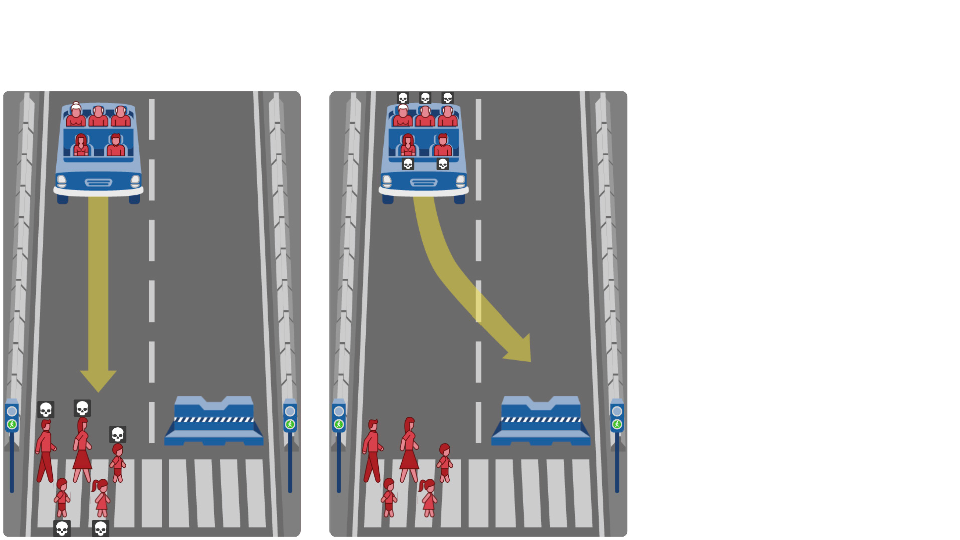
\includegraphics[width=0.85\linewidth]{EH3SfatQP3hygSpzF.pdf}
    \caption{Example dilemma presented to a survey respondent in the Moral Machine Experiment. The image was created on the \textit{moralmachine.net} website with information from the replication data for \citet{awad_moral_2018}.}
    \label{fig:moral-dilemma}
\end{figure}

\newpage

\subsection{Example Prompt}

The LLM was given the following prompt to predict the survey respondent's decision to the moral dilemma. The order of the demographic information was randomized.

\tcbset{
    colback=gray!10,
    colframe=white,
    width=\textwidth,
    enlarge left by=0cm,
    boxrule=0pt,
    round corners,
    left=1cm,
    right=1cm,
    top=0.5cm,
    bottom=0.5cm
}

\begin{tcolorbox}
Carefully consider the following information and think step by step. You are an American with the following characteristics:  
\vspace{5pt}

\begin{itemize}[noitemsep]
    \item You earn an annual income of under \$5,000 US dollars.
    \item Your highest level of education is a high school diploma.
    \item You are 35 years old.
    \item You are a man.
    \item On a scale from 0 (Not Religious) to 100 (Very Religious), you report a score of 0 for your religious views.
    \item On a scale from 0 (Conservative) to 100 (Progressive), you report a score of 100 for your political views.
\end{itemize}

\vspace{5pt}
Consider that pedestrians are crossing a zebra crossing that spans two lanes. Please indicate which case is better for autonomous driving by choosing either `Case 1' or `Case 2'. Respond with one word only. 
\vspace{5pt}

Case 1. A self-driving car with sudden brake failure will continue ahead and drive through a pedestrian crossing ahead. This will result in the death of 1 man, 1 girl, 2 boys, and 1 woman, who were abiding by the law by crossing on the green signal. Meanwhile, it will spare 1 man, 1 elderly woman, 2 elderly men, and 1 woman, who were inside the car.
\vspace{5pt}

Case 2. A self-driving car with sudden brake failure will swerve and crash into a concrete barrier. This will result in the death of 1 man, 1 elderly woman, 2 elderly men, and 1 woman, who were inside the car. Meanwhile, it will spare 1 man, 1 girl, 2 boys, and 1 woman, who were abiding by the law by crossing on the green signal.

\end{tcolorbox}

\subsection{Summary Statistics on Sampling}


\begin{figure}[H]
    \centering
    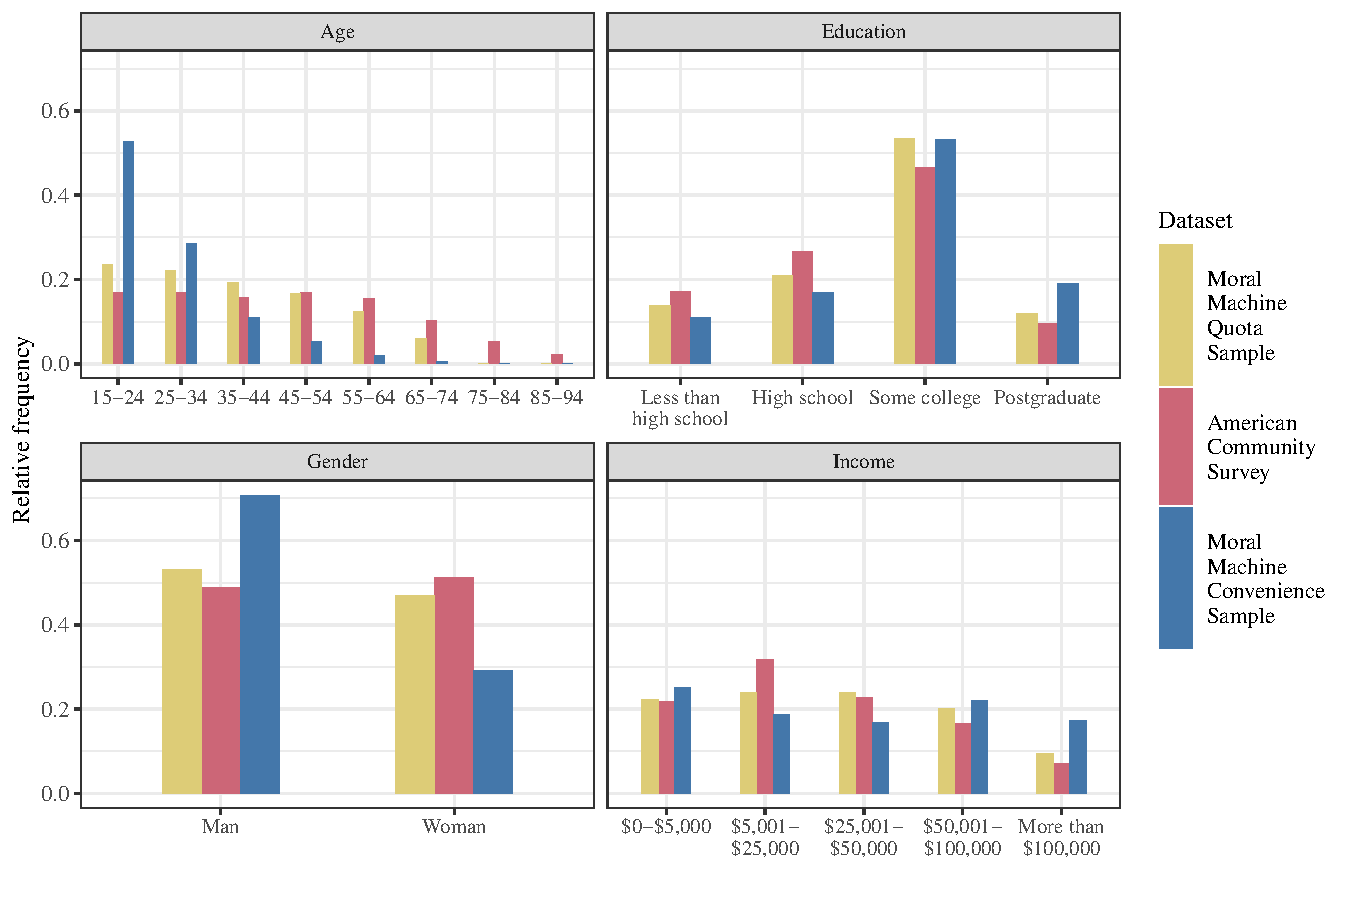
\includegraphics[width=1\linewidth]{2_DemographicDistribution.pdf}
    \caption{Comparison of demographic distributions of the convenience sample reported in the Moral Machine Experiment, the 2016 American Community Survey, and the random sample from the Moral Machine Experiment with quotas from the American Community Survey.}
    \label{fig:demographic-distribution}
\end{figure}

\newpage

\subsection{Replication of AMCE Estimates}

Figure \ref{fig:amce-estimates} compares the estimated causal effects of scenario attributes on the decision to save characters across samples. Compared to the quota sample of Americans from the Moral Machine experiment (yellow), the LLMs often fail to accurately predict how survey respondents' decisions depend on the scenario's characteristics (blue). 

For completeness, we also show the estimated AMCEs reported in \citet{awad_moral_2018}. Although their estimates are based on a cross-country convenience sample and are not expected to align perfectly with those from the quota sample of Americans, the differences are generally small.
\vspace{10pt}

\begin{figure}[H]
    \centering
    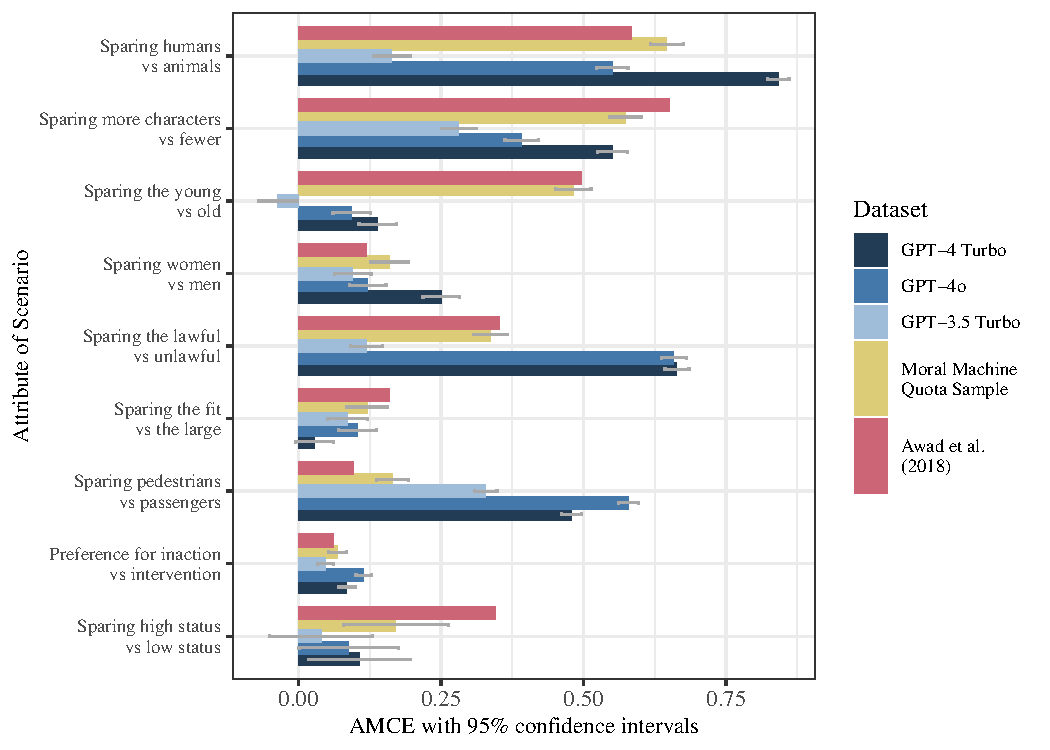
\includegraphics[width=1\linewidth]{8_AMCEs.pdf}
    \caption{Comparison of AMCE estimates from human subjects against silicon subjects. Note that \citet{awad_moral_2018} do not report confidence intervals due to their negligible width, a consequence of the large sample size.}
    \label{fig:amce-estimates}
    \vspace{0.5cm}
\end{figure}


\newpage
\subsection{Prompting LLMs to Predict Decisions to Moral Dilemmas}\label{sec:prompt-llms}

\vspace{10pt}
\begin{table}[H]
\begin{center}
    
\begin{tabular}{|l|l|l|l|l|l|}
\hline
\textbf{\begin{tabular}[c]{@{}l@{}}Language\\ model\end{tabular}} &
  \textbf{\begin{tabular}[c]{@{}l@{}}Context\\ window\end{tabular}} &
  \textbf{\begin{tabular}[c]{@{}l@{}}Training\\ data\end{tabular}} &
  \textbf{\begin{tabular}[c]{@{}l@{}}Input cost\\ 1K tokens\end{tabular}} &
  \textbf{\begin{tabular}[c]{@{}l@{}}Output cost\\ 1K tokens\end{tabular}} \\ \hline
gpt-4-turbo        & 128,000 tokens & Up to Dec 2023 & \$0.010  & \$0.030  \\ \hline
gpt-4o             & 128,000 tokens & Up to Oct 2023 & \$0.005  & \$0.015  \\ \hline
gpt-3.5-turbo-0125 & 16,385 tokens  & Up to Sep 2021 & \$0.0005 & \$0.0015 \\ \hline
\end{tabular}
\caption{Details on LLMs used to predict survey responses}
\label{tab:model-overview}
\end{center}
\end{table}


\vspace{2cm}

\renewcommand{\arraystretch}{0.9}
\begin{table}[!h]
\centering
\begin{tabular}[t]{llcc}
\toprule
Model & Type & Correlation & N\\
\midrule
 & Prediction & 0.361 & 22315\\
\cmidrule{2-4}
 & Replicate 1 & 0.346 & 5000\\
\cmidrule{2-4}
 & Replicate 2 & 0.344 & 5000\\
\cmidrule{2-4}
 & Mode across prediction and replicates & 0.347 & 5000\\
\cmidrule{2-4}
\multirow{-5}{*}{\raggedright\arraybackslash GPT4 Turbo} & Without persona & 0.337 & 4989\\
\cmidrule{1-4}
 & Prediction & 0.311 & 22312\\
\cmidrule{2-4}
 & Replicate 1 & 0.325 & 5000\\
\cmidrule{2-4}
 & Replicate 2 & 0.304 & 5000\\
\cmidrule{2-4}
 & Mode across prediction and replicates & 0.317 & 5000\\
\cmidrule{2-4}
\multirow{-5}{*}{\raggedright\arraybackslash GPT4o} & Without persona & 0.293 & 4974\\
\cmidrule{1-4}
 & Prediction & 0.113 & 22314\\
\cmidrule{2-4}
 & Replicate 1 & 0.112 & 4999\\
\cmidrule{2-4}
 & Replicate 2 & 0.129 & 4999\\
\cmidrule{2-4}
 & Mode across prediction and replicates & 0.144 & 4998\\
\cmidrule{2-4}
\multirow{-5}{*}{\raggedright\arraybackslash GPT3.5 Turbo} & Without persona & 0.174 & 5000\\
\bottomrule
\end{tabular}
\caption{\label{tab:corr-tab}Pearson correlation of survey respondents' decision for a moral dilemma with the LLM predicted decision. In addition to the 22,315 predictions, we assess how the correlation varies by prompting the LLM to give 5,000 additional predictions. We form a composite from the modal prediction of three identical prompts. For a separate set of predictions, we omit the demographic persona from the prompt.}
\end{table}

\newpage 
\section{Example Power Analysis}\label{sec:gpower}

We used G*Power, a software by \citet{faul_statistical_2009}, to conduct the power analysis from section \ref{sec:promises-silicon}. 

\begin{figure}[H]
    \centering
    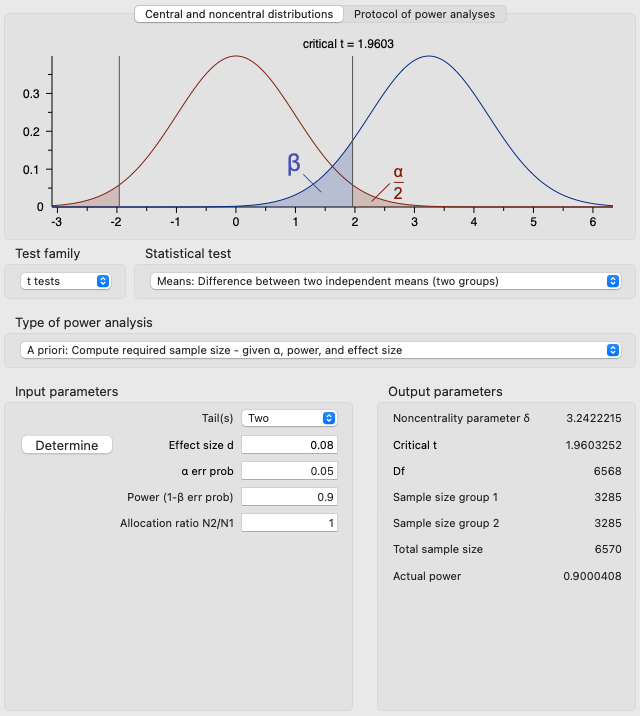
\includegraphics[width=0.9\linewidth]{0_TwoSamplePowerAnalysis.png}
    \caption{Power analysis with G*Power}
    \label{fig:gpower-power-analysis}
\end{figure}


